% !TeX root = ../../Skript.tex
\cohead{\Large\textbf{Vermischte Aufgaben}}
\fakesubsection{Vermischte Aufgaben}
Die folgenden Aufgaben sind Aufgaben aus alten Abschlussprüfungen nachempfunden. Es ist jeweils angegeben, wie viel Zeit in der Abschlussprüfung zur Bearbeitung der Aufgabe zur Verfügung stehen würde.
\begin{Exercise}[title={Zeitansatz 8 min, ohne Taschenrechner}, label=eFktVA_1]%2018-1.3

Lösen Sie die Gleichung \(e^{2x}-4e^x=0\)
\end{Exercise}
\begin{Exercise}[title={Zeitansatz 10 min, ohne Taschenrechner}, label=eFktVA_2]%2018-1.4

    \begin{minipage}{\textwidth}
        \adjustbox{valign=t, padding=0ex 0ex 2ex 0ex}{\begin{minipage}{0.5\textwidth-2ex}
            Gegeben ist die Funktion \(f\) mit

            \(f(x)=a\cdot e^{-x}+b,\ x\in\R;\ a,b\neq0\)

            Begründen Sie, welches der Schaubilder \(S_1\) oder \(S_2\) zur Funktion \(f\) gehört.

            Bestimmen Sie \(a\) und \(b\).
        \end{minipage}}%
        \adjustbox{valign=t, padding=2ex 0ex 0ex 0ex}{\begin{minipage}{0.5\textwidth-2ex}\centering
            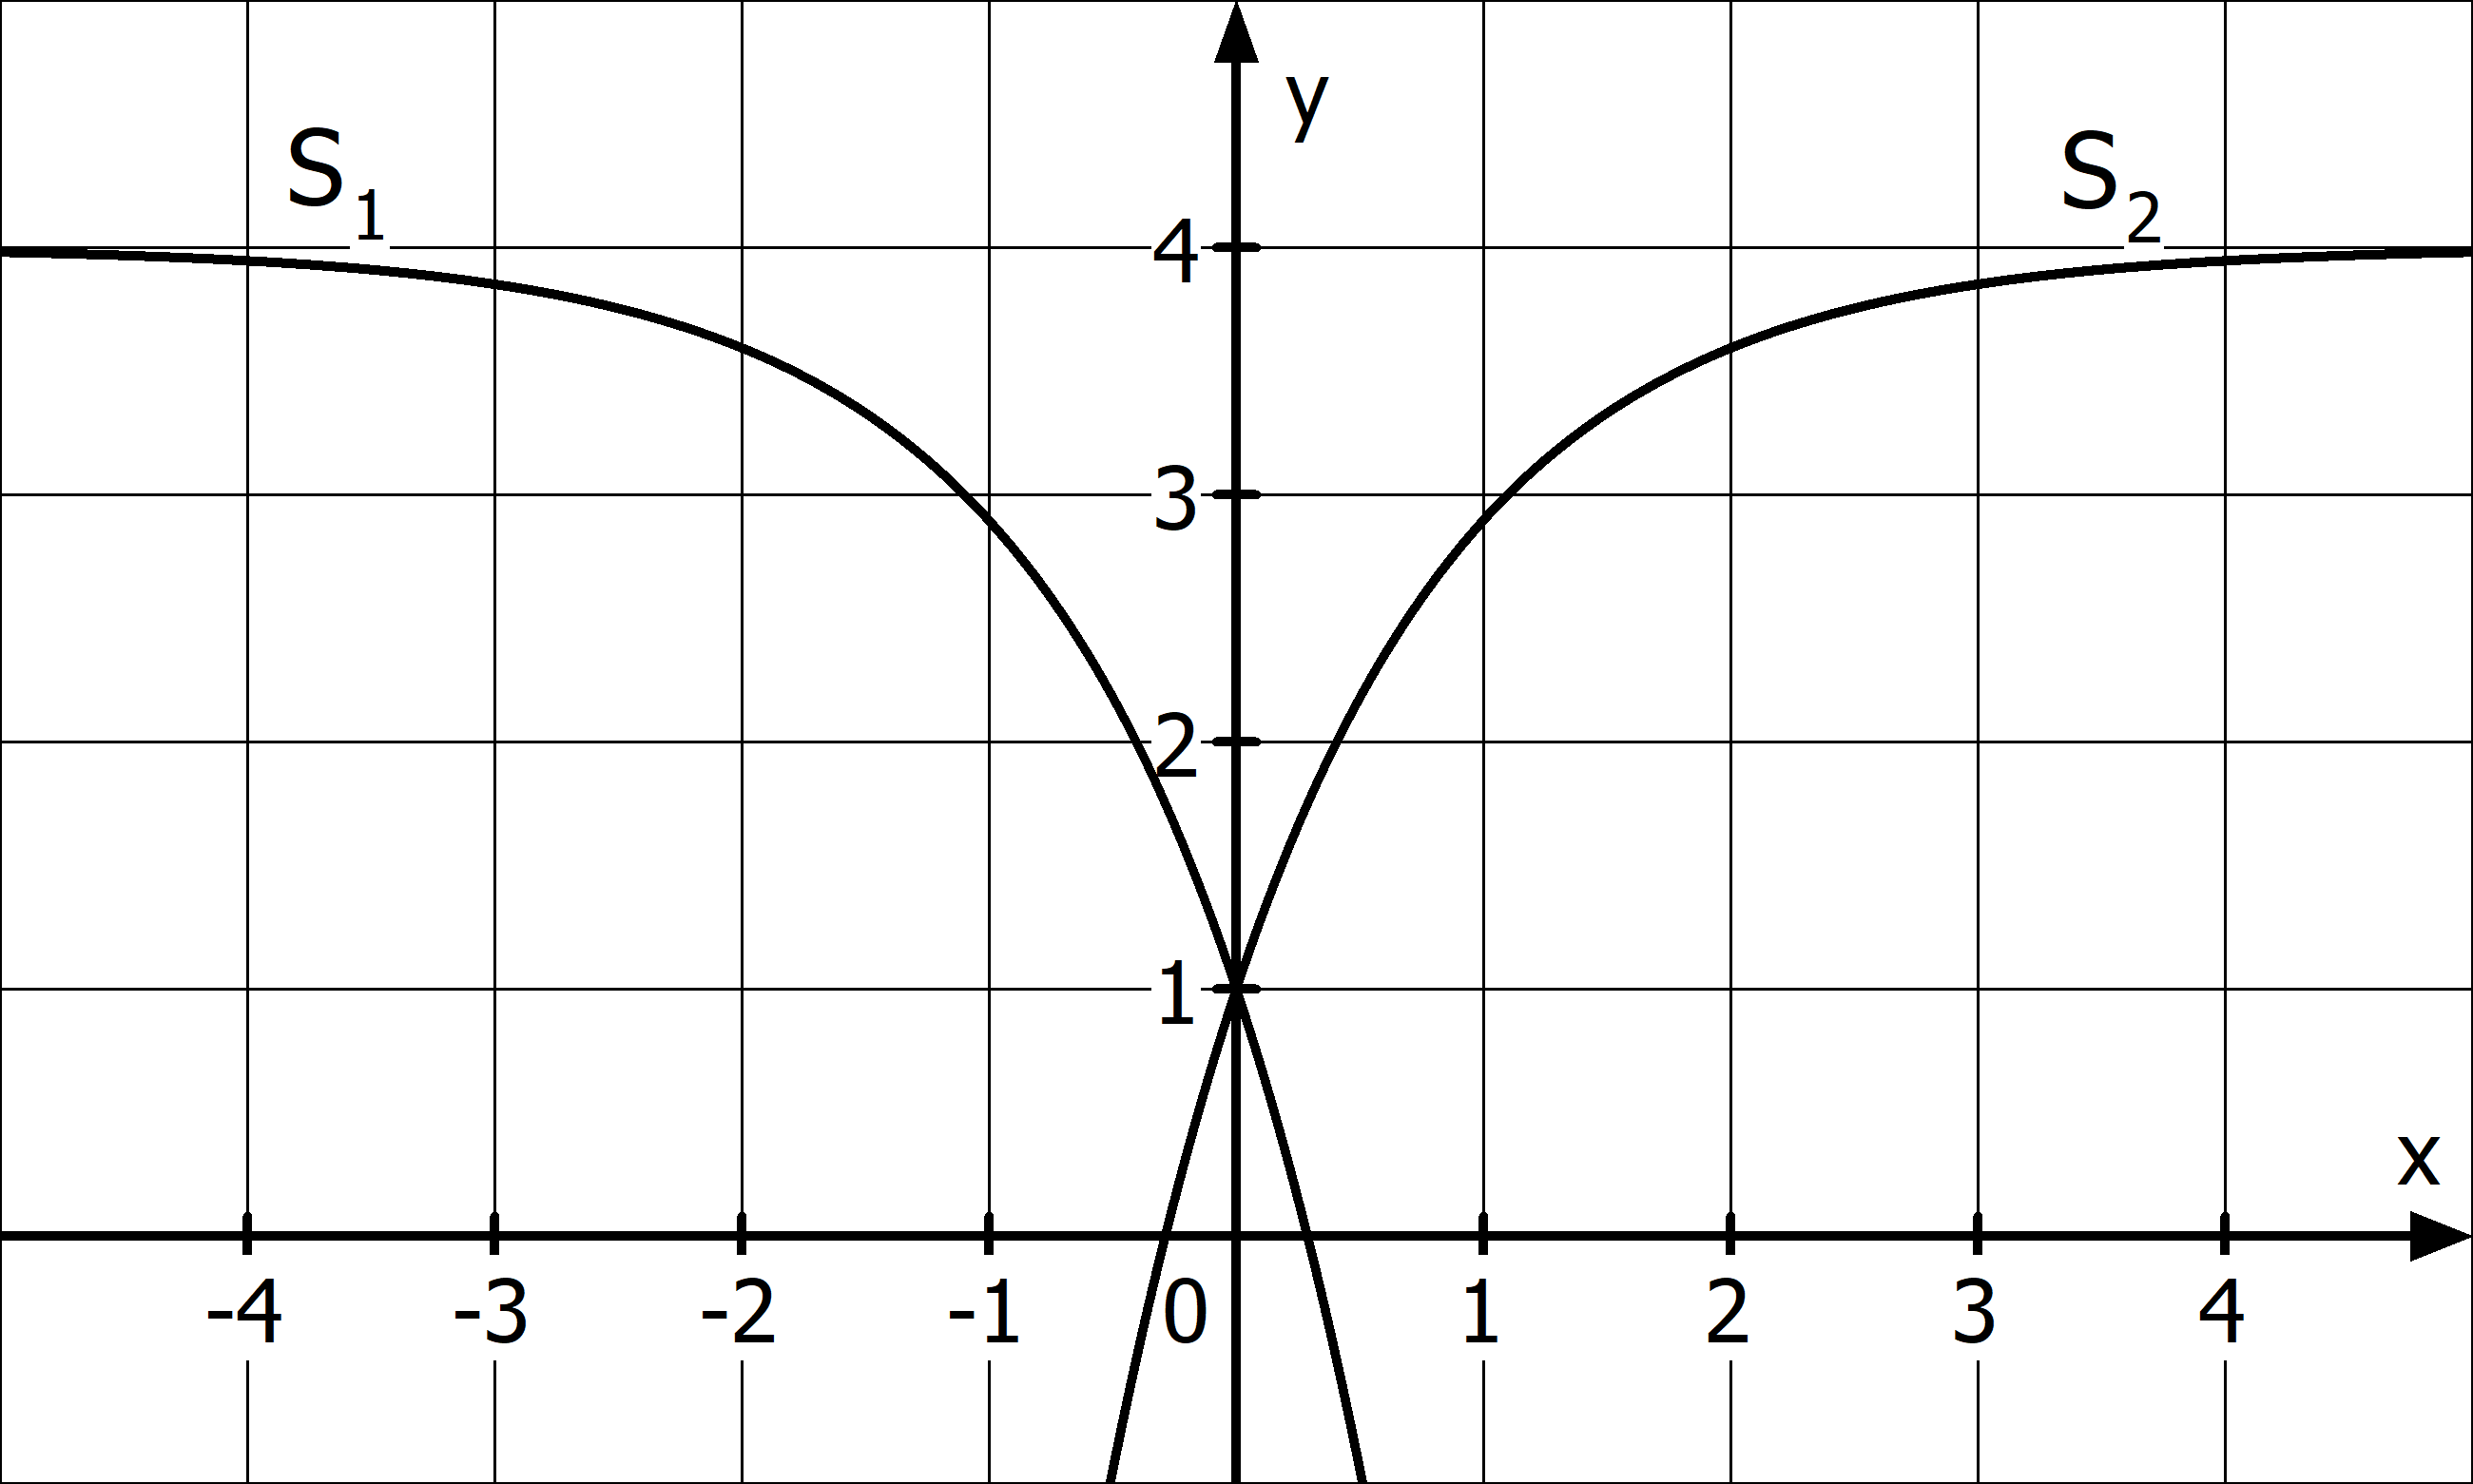
\includegraphics[width=\textwidth]{\eFkt/pics/VA_2.png}
        \end{minipage}}%
    \end{minipage}
\end{Exercise}
\begin{Exercise}[title={Zeitansatz 20 min, mit Taschenrechner}, label=eFktVA_3]%2018-2.4 bis 2.6

    Die Einwohnerzahl eines Landes wird durch die Funktion \(f\) dargestellt mit

    \(f(x)=a\cdot e^{b\cdot t}\) mit \(t\in\R;\ a,b\neq0\)

    Dabei ist \(t\) die Zeit in Jahren, \(t=0\) entspricht dem Jahr 2020 und \(f(t)\) gibt die Einwohnerzahl in Millionen zum Zeitpunkt \(t\) an.

    2020 lebten 85 Millionen Menschen im Land, 2023 waren es 97 Millionen.

    \begin{enumerate}[label=\alph*)]
        \item (6 Minuten) Bestimmen Sie \(a\) und \(b\).
    \end{enumerate}

    Im Folgenden sei \(a=85\) und \(b=0,044\).

    \begin{enumerate}[label=\alph*)]
        \setcounter{enumi}{1}
        \item (8 Minuten) Bestimmen Sie die Bevölkerungszahl im Jahr 2030.

        In welchem Jahr betrug die Bevölkerungszahl Drei Viertel der Bevölkerungszahl im Jahr 2020?
        \item (6 Minuten) Bestimmen Sie, um wie viel Prozent die Bevölkerung pro Jahr wächst.
    \end{enumerate}
\end{Exercise}
\begin{Exercise}[title={Zeitansatz 6 min, mit Taschenrechner}, label=eFktVA_4]%2018-3.1

    Berechnen Sie die Koordinaten der Achsenschnittpunkte des Schaubildes von \(f(x)=-3e^{-0,25x}+5\)
\end{Exercise}
\begin{Exercise}[title={Zeitansatz 10 min, ohne Taschenrechner}, label=eFktVA_5]%2019-1.5

    Die Funktion \(g\) ist gegeben durch \(g(x)=3e^{-x}-2,\ x\in\R\).

    Das Schaubild heißt \(K_g\). Geben Sie die Gleichung der Asymptoten von \(K_g\) an und skizzieren Sie \(K_g\).

    Gib den Quadranten an, in dem \(K_g\) mit den Koordinatenachsen eine Fläche einschließt.
\end{Exercise}
\begin{Exercise}[title={Zeitansatz 6 min, ohne Taschenrechner}, label=eFktVA_6]%2020-1.3

    Lösen Sie die Gleichung \(4e^{-3x}-8=0\)
\end{Exercise}
\begin{Exercise}[title={Zeitansatz 26 min, mit Taschenrechner}, label=eFktVA_7]%2020-2.4 und 2.5

    Eine Grippe verbreitet sich in der Bevölkerung. Die Funktion \(g(t)=-90e^{-0,014t}+90,\ t\geq0\)

    beschreibt den Anteil der Bevölkerung, die infiziert wurde, in Prozent nach \(t\) Tagen, \(t=0\) entspricht dem 3. März 2023.
    \begin{enumerate}[label=\alph*)]
        \item Skizzieren Sie das Schaubild von \(g\).
        \item Wie viel Prozent der Bevölkerung werden sich nie infizieren?
        \item Ermitteln Sie den Anteil der Bevölkerung, der sich nach 70 Tagen infiziert hat.
        \item Zu welchem Zeitpunkt hat sich die Hälfte der Bevölkerung infiziert?
    \end{enumerate}
    Zeitgleich zum Ausbruch der Grippe wird eine Infektion mit Fußpilz festgestellt, die große Teile der Bevölkerung betrifft, aber leicht behandelbar ist. Die Funktion \(h\) mit \(h(t)=a\cdot e^{b\cdot t}+10,\ t\geq0,\ a,b\neq0\) beschreibt den Anteil der mit Fußpilz infizierten.
    \begin{itemize}
        \item Zum Zeitpunkt \(t=0\) sind 60\% der Bevölkerung mit Fußpilz infiziert.
        \item Nach 20 Tagen sind die Anteile der Bevölkerung, die mit der Grippe infiziert wurde und die unter Fußpilz leiden, gleich groß.
    \end{itemize}
    Bestimmen Sie Werte für \(a\) und \(b\).
\end{Exercise}
\begin{Exercise}[title={Zeitansatz 14 min, mit Taschenrechner}, label=eFktVA_8]%2020-3.1 und 3.2

    Gegeben ist die Funktion \(f\) mit \(f(x)=0,75e^{0,4x}-x+1,25,\ x\in\R\).

    Ihr Schaubild ist \(K_f\).
    \begin{enumerate}[label=\alph*)]
        \item Zeichnen Sie \(K_f\) für \(-3\leq x\leq 7\).
        \item Das Schaubild \(K_f\) wird so verschoben, dass es durch den Urpsrung verläuft. Geben Sie einen neuen Funktionsterm \(f_v(x)\) an.
    \end{enumerate}
\end{Exercise}
\begin{Exercise}[title={Zeitansatz 4 min, ohne Taschenrechner}, label=eFktVA_9]%2021-1.4V2

    Weisen Sie nach, dass die Funktion \(k(x)=3e^{4x}+4x-6\) zwischen \(x=0\) und \(x=0,25\) eine Nullstelle besitzt.
\end{Exercise}
\begin{Exercise}[title={Zeitansatz 10 min, mit Taschenrechner}, label=eFktVA_10]%2021-2.4 bis 2.6

In einem chemischen Experiment wird eine Flüssigkeit mit Kalilauge titriert. Der pH-Wert der Flüssigkeit wird mit einem Messgerät erfasst durch die Funktion \(p(V)=13,5-6,5e^{-0,2V},\ V\geq0\) beschrieben, dabei ist \(V\) das Volumen der hinzugefügten Kalilauge in Millilitern.
\begin{enumerate}[label=\alph*)]
    \item Geben Sie den Bereich an, den das ph-Wert-Messgerät für diesen Versuch abdecken muss.
    \item Bei einem ph-Wert von 10 schlägt ein Indikator um und die Farbe der Flüssigkeit ändert sich. Bestimmen Sie das Volumen der hinzugefügten Kalilauge am Umschlagpunkt.
\end{enumerate}
\end{Exercise}
\begin{Exercise}[title={Zeitansatz 8 min, ohne Taschenrechner}, label=eFktVA_11]%2022-1.3V1

Lösen Sie die Gleichung \(e^{-2x}-4e^{-x}=0\)
\end{Exercise}
\begin{Exercise}[title={Zeitansatz 6 min, ohne Taschenrechner}, label=eFktVA_12]%2022-1.4V2

Lösen Sie die Gleichung \(2e^x-4=e^x\)
\end{Exercise}
\begin{Exercise}[title={Zeitansatz 10 min, mit Taschenrechner}, label=eFktVA_13]%2022-3.1

Gegeben ist die Funktion \(f\) mit \(f(x)=1,5e^{-0,25x}-4,\ x\in\R\).

Ihr Schaubild ist \(K_f\).
\begin{itemize}
    \item Bestimmen Sie die Gleichung der Asymptoten von \(K_f\).
    \item Zeichnen Sie \(K_f\) für \(-6\leq x\leq8\).
    \item Wie müsste \(K_f\) verschoben werden, sodass das verschobene Schaubild die Asymptote \(y_v=2\) hat?
\end{itemize}
\end{Exercise}
\begin{Exercise}[title={Zeitansatz 8 min, ohne Taschenrechner}, label=eFktVA_14]%2023-1.7V2

Das Schaubild einer Funktion \(g\) wird nacheinander
\begin{enumerate}
    \item mit dem Faktor 2 in y-Richtung gestreckt
    \item um 3 Längeneinheiten in \(y\)-Richtung nach unten verschoben.
\end{enumerate}
Es ergibt sich auf diese Weise das Schaubild einer Funktion \(h\) mit

\(h(x)=6e^{-2x}+4\)

Geben Sie den Funktionsterm von \(g\) an.
\end{Exercise}
\begin{Exercise}[title={Zeitansatz 28 min, mit Taschenrechner}, label=eFktVA_15]%2023-3.1 bis 3.4

An einem sonnigen Wintertag bereitet das Ehepaar Schmidt 2 Kaffee zu. Eine Person bleibt mit ihrem Kaffee in der Wohnung, die andere setzt sich nach draußen. Die Funktionen \(T_1\) und \(T_2\) beschreiben die Temperatur der beiden Kaffee in °C nach \(t\) Minuten nach der Zubereitung des Kaffees:

\(T_1(t)=21+68e^{-0,12t}\) und \(T_2(t)=-8+a\cdot e^{-0,12t},\ t\in[0;20]\)

Es gilt \(a=97\).
\begin{enumerate}[label=\alph*)]
    \item Begründen Sie, warum \(a\) den angegebenen Wert haben muss.
    \item Zeichnen Sie die Schaubilder beider Funktionen in ein Koordinatensystem.
    \item Welche der beiden Funktionen beschreibt die Temperatur des Kaffees in der Wohnung, welche die des Kaffees im Außenbereich. Begründen Sie ihre Wahl.
    \item Ab einer Temperatur von 45°C kann der Kaffee getrunken werden. Wie viele Minuten früher kann einer der Ehepartner seinen Kaffee genießen?
\end{enumerate}
\end{Exercise}
\newpage
%%%%%%%%%%%%%%%%%%%%%%%%%%%%%%%%%%%%%%%%%
\begin{Answer}[ref=eFktVA_1]
    \begin{align*}
        e^{2x}-4e^x&=0\\
        e^x\left(e^x-4\right)&=0\ \vert\ \text{SvN }e^x=0\Lightning\text{ oder}\\
        e^x-4&=0\ \vert\ +4\\
        e^x&=4\ \vert\ \ln\\
        x&=\ln(4)
    \end{align*}
\end{Answer}
\begin{Answer}[ref=eFktVA_2]

    Schaubilder vom Typ \(a\cdot e^{kx}+b\) verlaufen für positive \(k\) nach links gegen ihre Asymptote und nach rechts gegen \(\pm\infty\) (je nach Vorzeichen von \(a\)). Für negative \(k\) dreht sich dieses Verhalten gerade um. Da für die gegebene Funktion \(k=-1\) gilt, muss das Schaubild \(S_2\) das korrekte sein.

    Die Asymptote \(y=4\) kann abgelesen werden. Daher gilt \(b=4\).

    Aus dem \(y\)-Achsenabschnitt \(f(0)=1\) ergibt sich \(a+4=1\) und damit \(a=-3\).
\end{Answer}
\begin{Answer}[ref=eFktVA_3]
    \begin{enumerate}[label=\alph*)]
        \item Aus den Angaben 2020, also \(t=0\) lebten 85 Millionen Menschen im Land und 2023, also \(t=3\) lebten 97 Millionen im Land kann man zwei Gleichungen aufstellen:

        \(f(0)=85\) also \(a=85\)

        \(f(3)=97\) also \(b=\frac{1}{3}\ln\left(\frac{97}{85}\right)\)
        \item Im Jahr 2030 (\(t=10\)) leben 132 Millionen Menschen im Land, da \(f(10)=85e^{0,044\cdot10}\approx 132\).

        Drei Viertel von 85 Millionen entspricht 63,75 Millionen, da \(\frac{3}{4}\cdot 85=63,75\).
        \begin{align*}
            f(t)&=63,75\\
            85e^{0,044t}&=63,75\ \vert\ :85\\
            e^{0,044t}&=0,75\ \vert\ \ln\\
            0,044t&=\ln(0,75)\ \vert\ :0,044\\
            t&=\frac{250}{11}\ln(0,75)\\
            t&\approx-6,5
        \end{align*}
        Also betrug die Einwohnerzahl im Jahr 2013 (\(2020-6,5=2013,5\)) Drei Viertel der Bevölkerungszahl aus 2020.
        \item Bereits bekannt ist \(f(0)=85\). Mit \(f(1)=85e^{0,044}\approx88,82\) ergibt sich:

        \(\frac{88,82}{85}\approx1,045=104,5\%\)

        Die Bevölkerung wächst also jährlich um 4,5\%.
    \end{enumerate}
\end{Answer}
\begin{Answer}[ref=eFktVA_4]

    Schnittpunkt mit der \(y\)-Achse: \(f(0)=-3+5=2\), also \(S_y(0\vert2)\)

    Schnittpunkt mit der \(x\)-Achse:
    \begin{align*}
        f(x)&=0\\
        -3e^{-0,25x}+5&=0\ \vert\ -5\\
        -3e^{-0,25x}&=-5\ \vert\ :(-3)\\
        e^{-0,25x}&=\frac{5}{3}\ \big\vert\ \ln\\
        -0,25x&=\ln\left(\frac{5}{3}\right)\ \big\vert\ \cdot(-4)\\
        x&=-4\ln\left(\frac{5}{3}\right)
    \end{align*}

    \medskip

    Also ist der Schnittpunkt mit der \(x\)-Achse \(S_x\left(-4\ln\left(\frac{5}{3}\right)\middle\vert0\right)\)
\end{Answer}
\begin{Answer}[ref=eFktVA_5]

    \begin{minipage}{\textwidth}
        \adjustbox{valign=t, padding=0ex 0ex 2ex 0ex}{\begin{minipage}{0.7\textwidth-2ex}
                Asymptote: \(y=-2\)

                \(y\)-Achsenabschnitt für die Skizze: \(g(0)=3-2=1\)

                Die Fläche wird im 1. Quadranten eingeschlossen. (Die fast dreieckige Fläche zwischen dem \(y\)-Achsenabschnitt, dem Schnittpunkt mit der \(x\)-Achse und dem Ursprung.)
        \end{minipage}}%
        \adjustbox{valign=t, padding=2ex 0ex 0ex 0ex}{\begin{minipage}{0.3\textwidth-2ex}\centering
                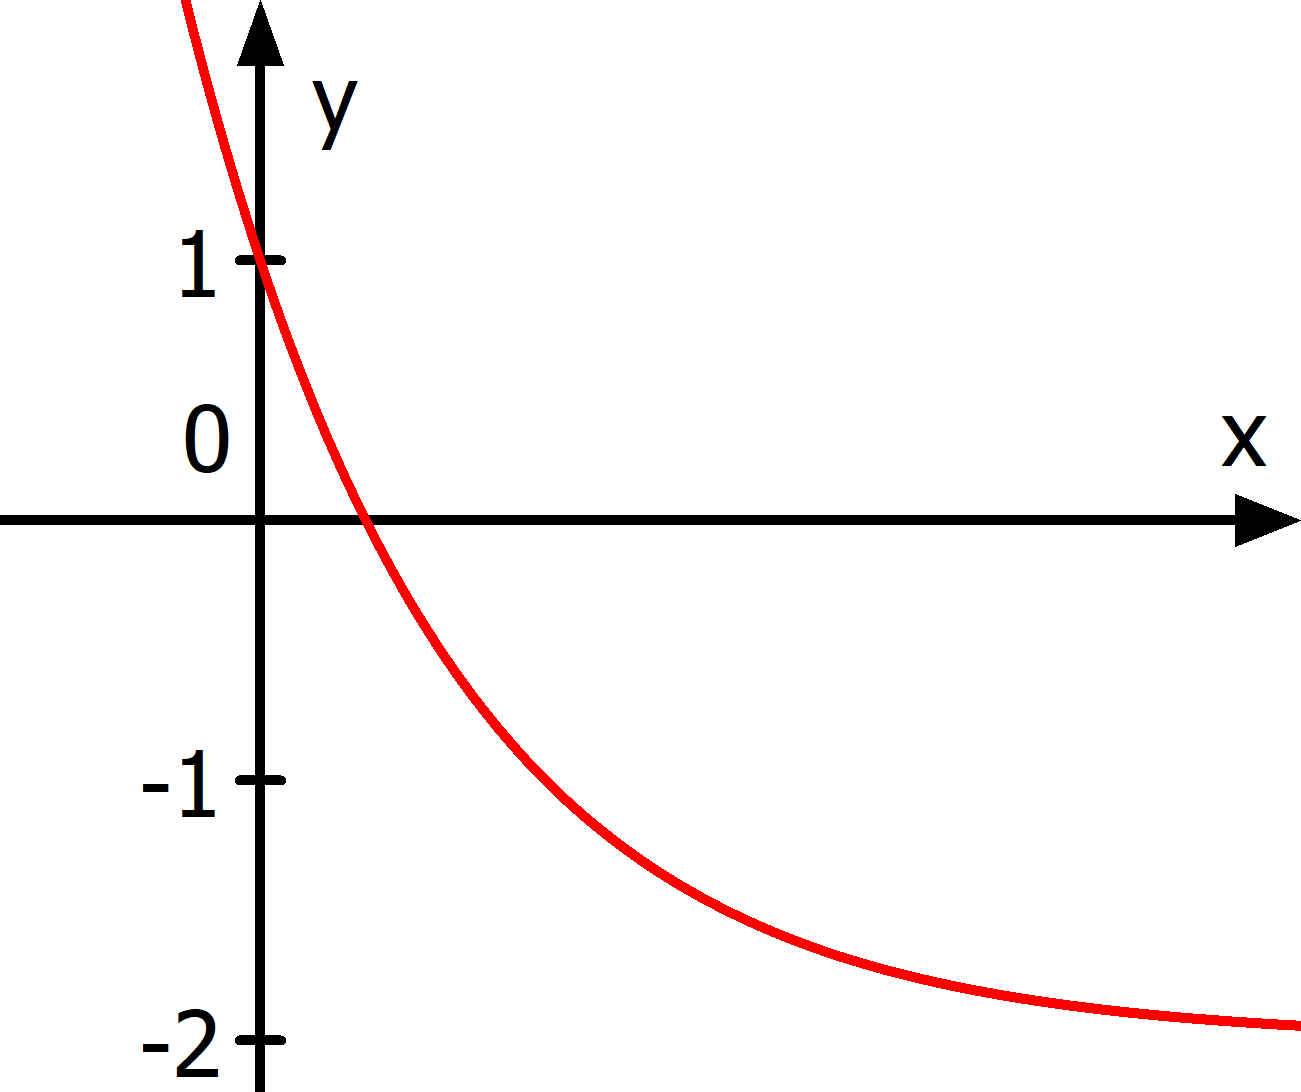
\includegraphics[width=\textwidth]{\eFkt/pics/VA_5.png}
        \end{minipage}}%
    \end{minipage}
\end{Answer}
\begin{Answer}[ref=eFktVA_6]
    \begin{align*}
        4e^{-3x}-8&=0\ \vert\ +8\\
        4e^{-3x}&=8\ \vert\ :4\\
        e^{-3x}&=2\ \vert\ \ln\\
        -3x&=\ln(2)\ \vert\ :(-3)\\
        x&=-\frac{\ln(2)}{3}
    \end{align*}
\end{Answer}
\begin{Answer}[ref=eFktVA_7]
    \begin{enumerate}[label=\alph*)]
        \item \(y\)-Achsenabschnitt: \(g(0)=-90+90=0\)

        \adjustbox{valign=t}{\begin{minipage}{.5\textwidth}\centering
                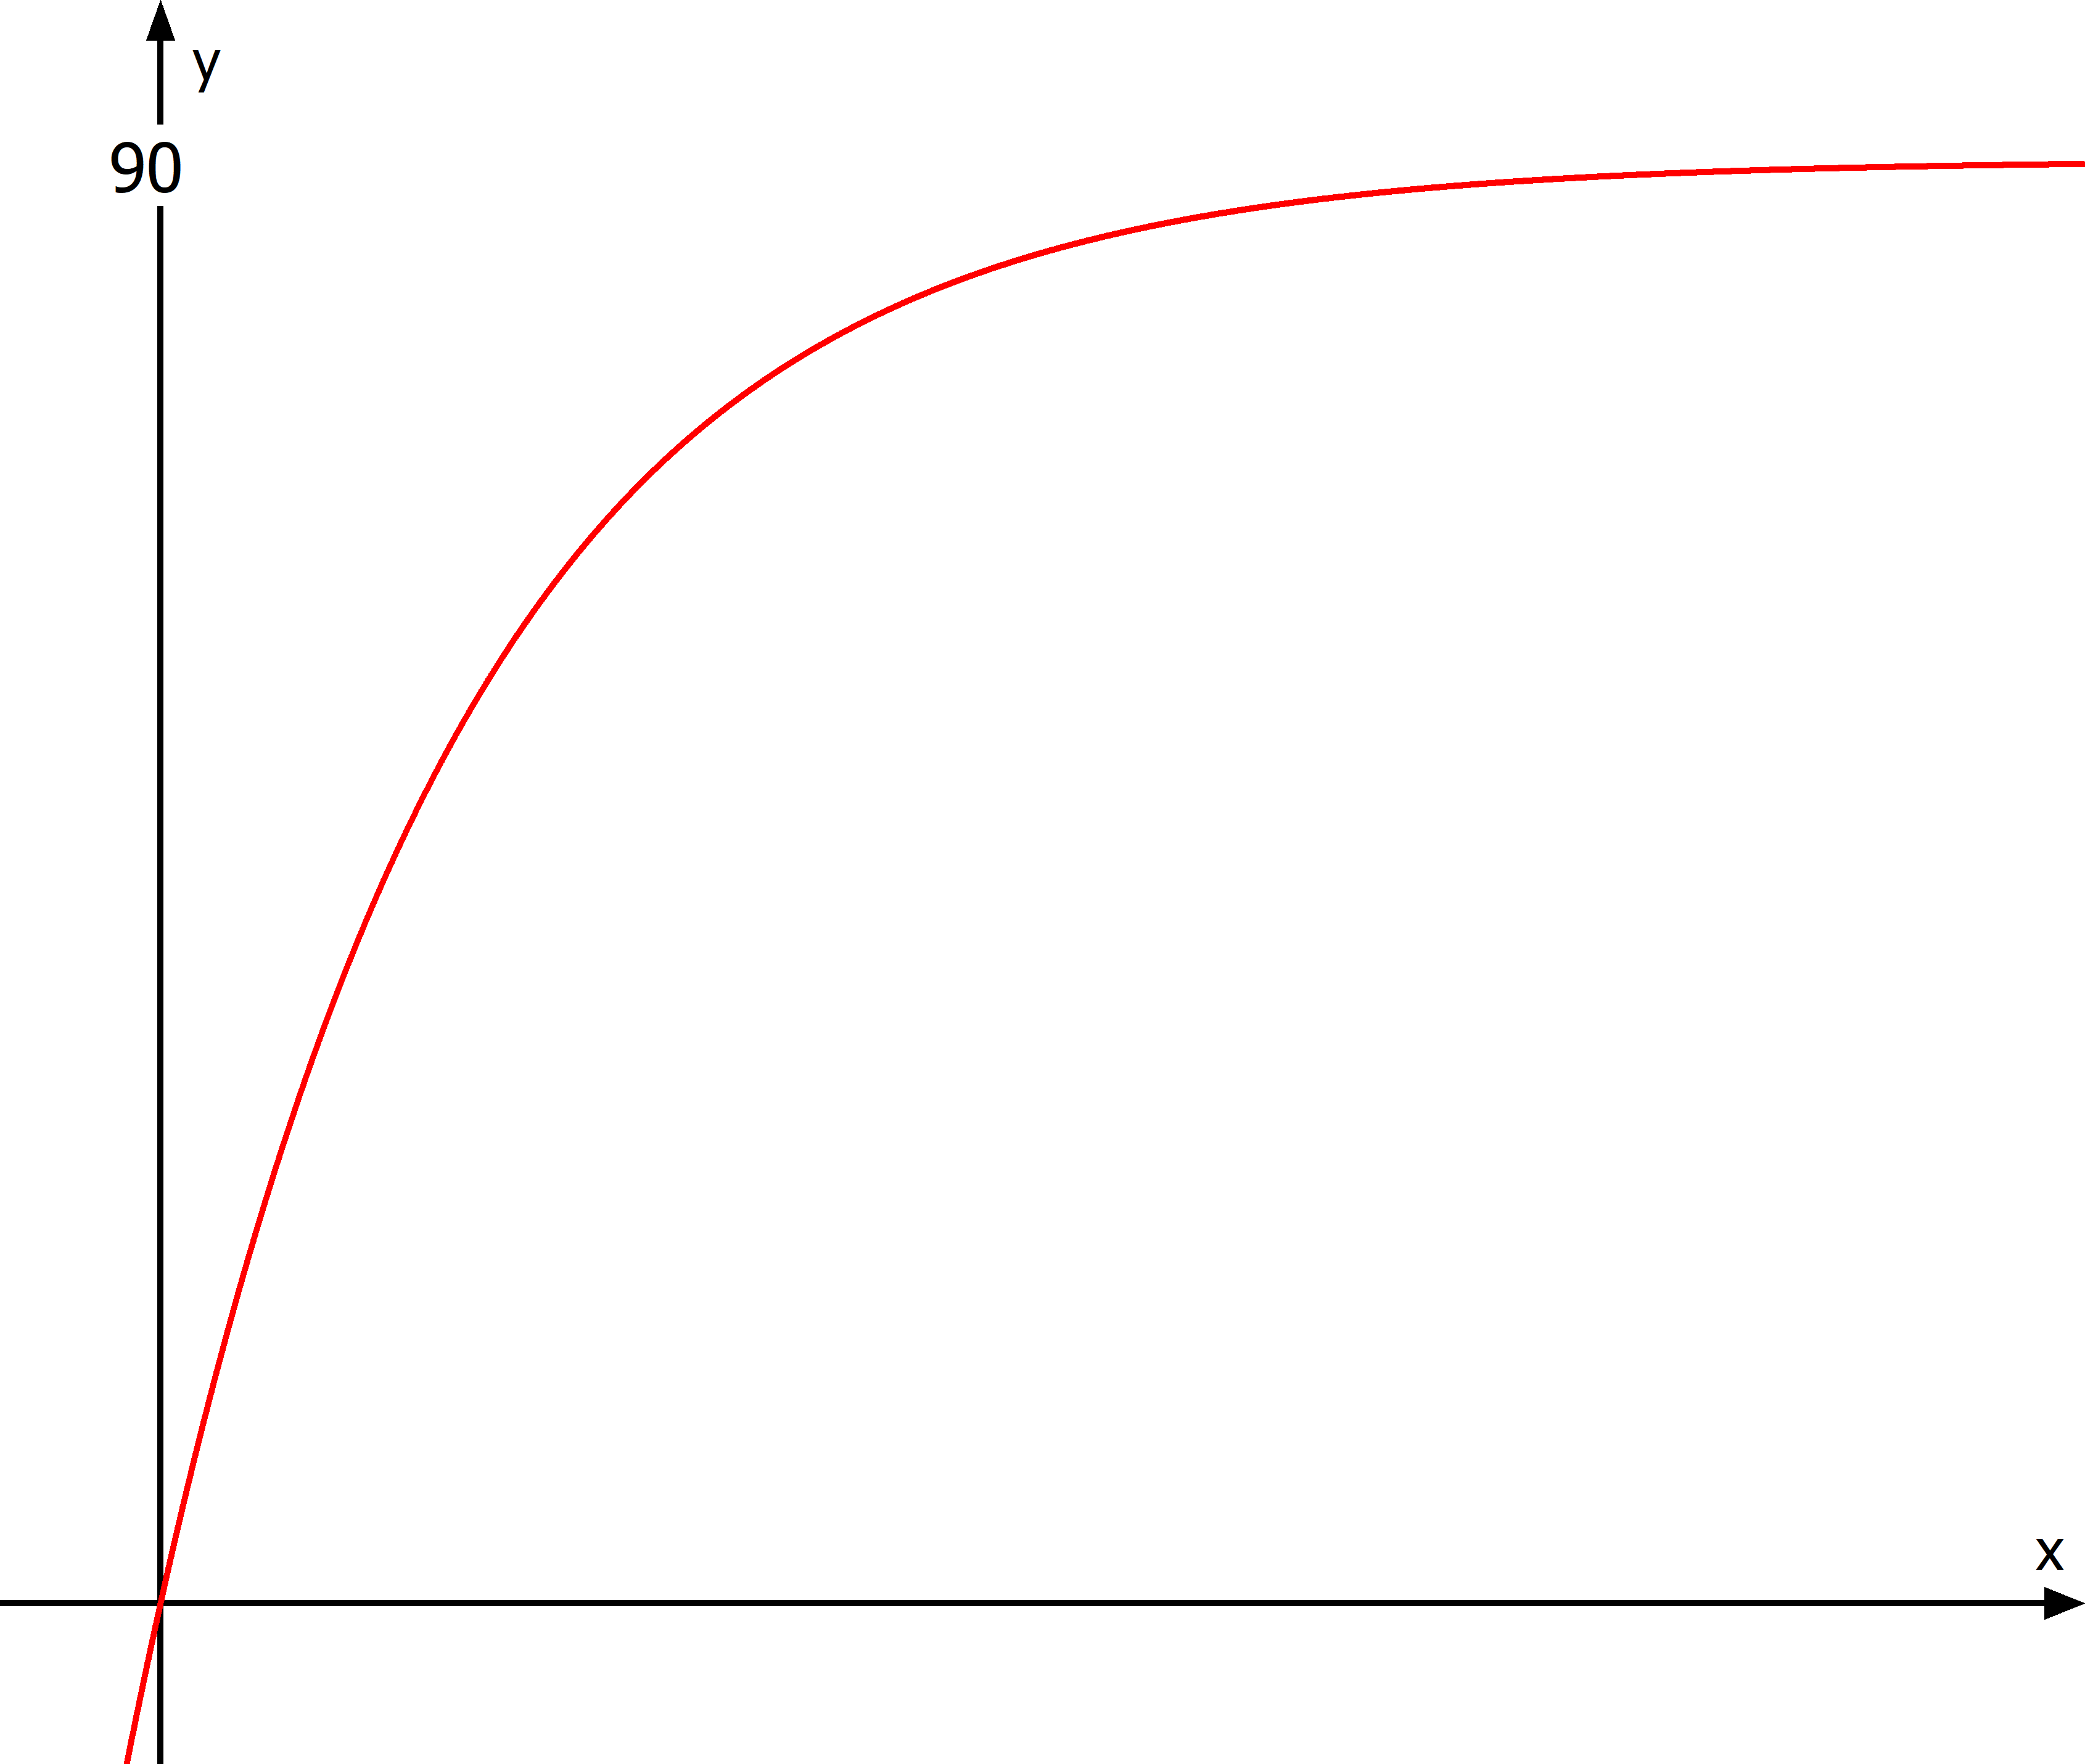
\includegraphics[width=\textwidth]{\eFkt/pics/VA_7.png}
        \end{minipage}}%
        \item Da der Anteil der Infizierten gegen die Asymptote von \(y=90\) strebt, werden sich die verbleibenden 10\% nie infizieren.
        \item Nach 70 Tagen haben sich ca 56\% infiziert, da \(g(70)\approx 56\).
        \item Die Hälfte der Bevölkerung wird sich nach 58 Tagen, als am 30. April 2023, infiziert haben:
        \begin{align*}
            g(t)&=50\\
            -90e^{-0,014t}+90&=50\ \vert\ -90\\
            -90e^{-0,014t}&=-40\ \vert\ :(-90)\\
            e^{-0,014t}&=\frac{4}{9}\ \big\vert\ \ln\\
            -0,014t&=\ln\left(\frac{4}{9}\right)\ \big\vert\ :(-0,014)\\
            t&\approx58
        \end{align*}
    \end{enumerate}
    Da zu Beginn 60\% infiziert sind, ergibt sich \(h(0)=60\), also \(a=60\).

    Nach 20 Tagen beträgt der Anteil, der unter der Grippe leidet \(g(20)\approx22\),

    also muss auch \(h(20)=22\) gelten:
    \begin{align*}
        h(20)&=22\\
        60\cdot e^{b\cdot 20}&=22\ \vert\ :60\\
        e^{b\cdot 20}&=\frac{11}{30}\ \vert\ \ln\\
        b\cdot 20&=\ln\left(\frac{11}{30}\right)\ \vert\ :20\\
        b&=\frac{1}{20}\ln\left(\frac{11}{30}\right)
    \end{align*}
\end{Answer}
\begin{Answer}[ref=eFktVA_8]
    \begin{enumerate}[label=\alph*)]
        \item Wertetabelle im Taschenrechner verwenden:

        \adjustbox{valign=t}{\begin{minipage}{.5\textwidth}\centering
                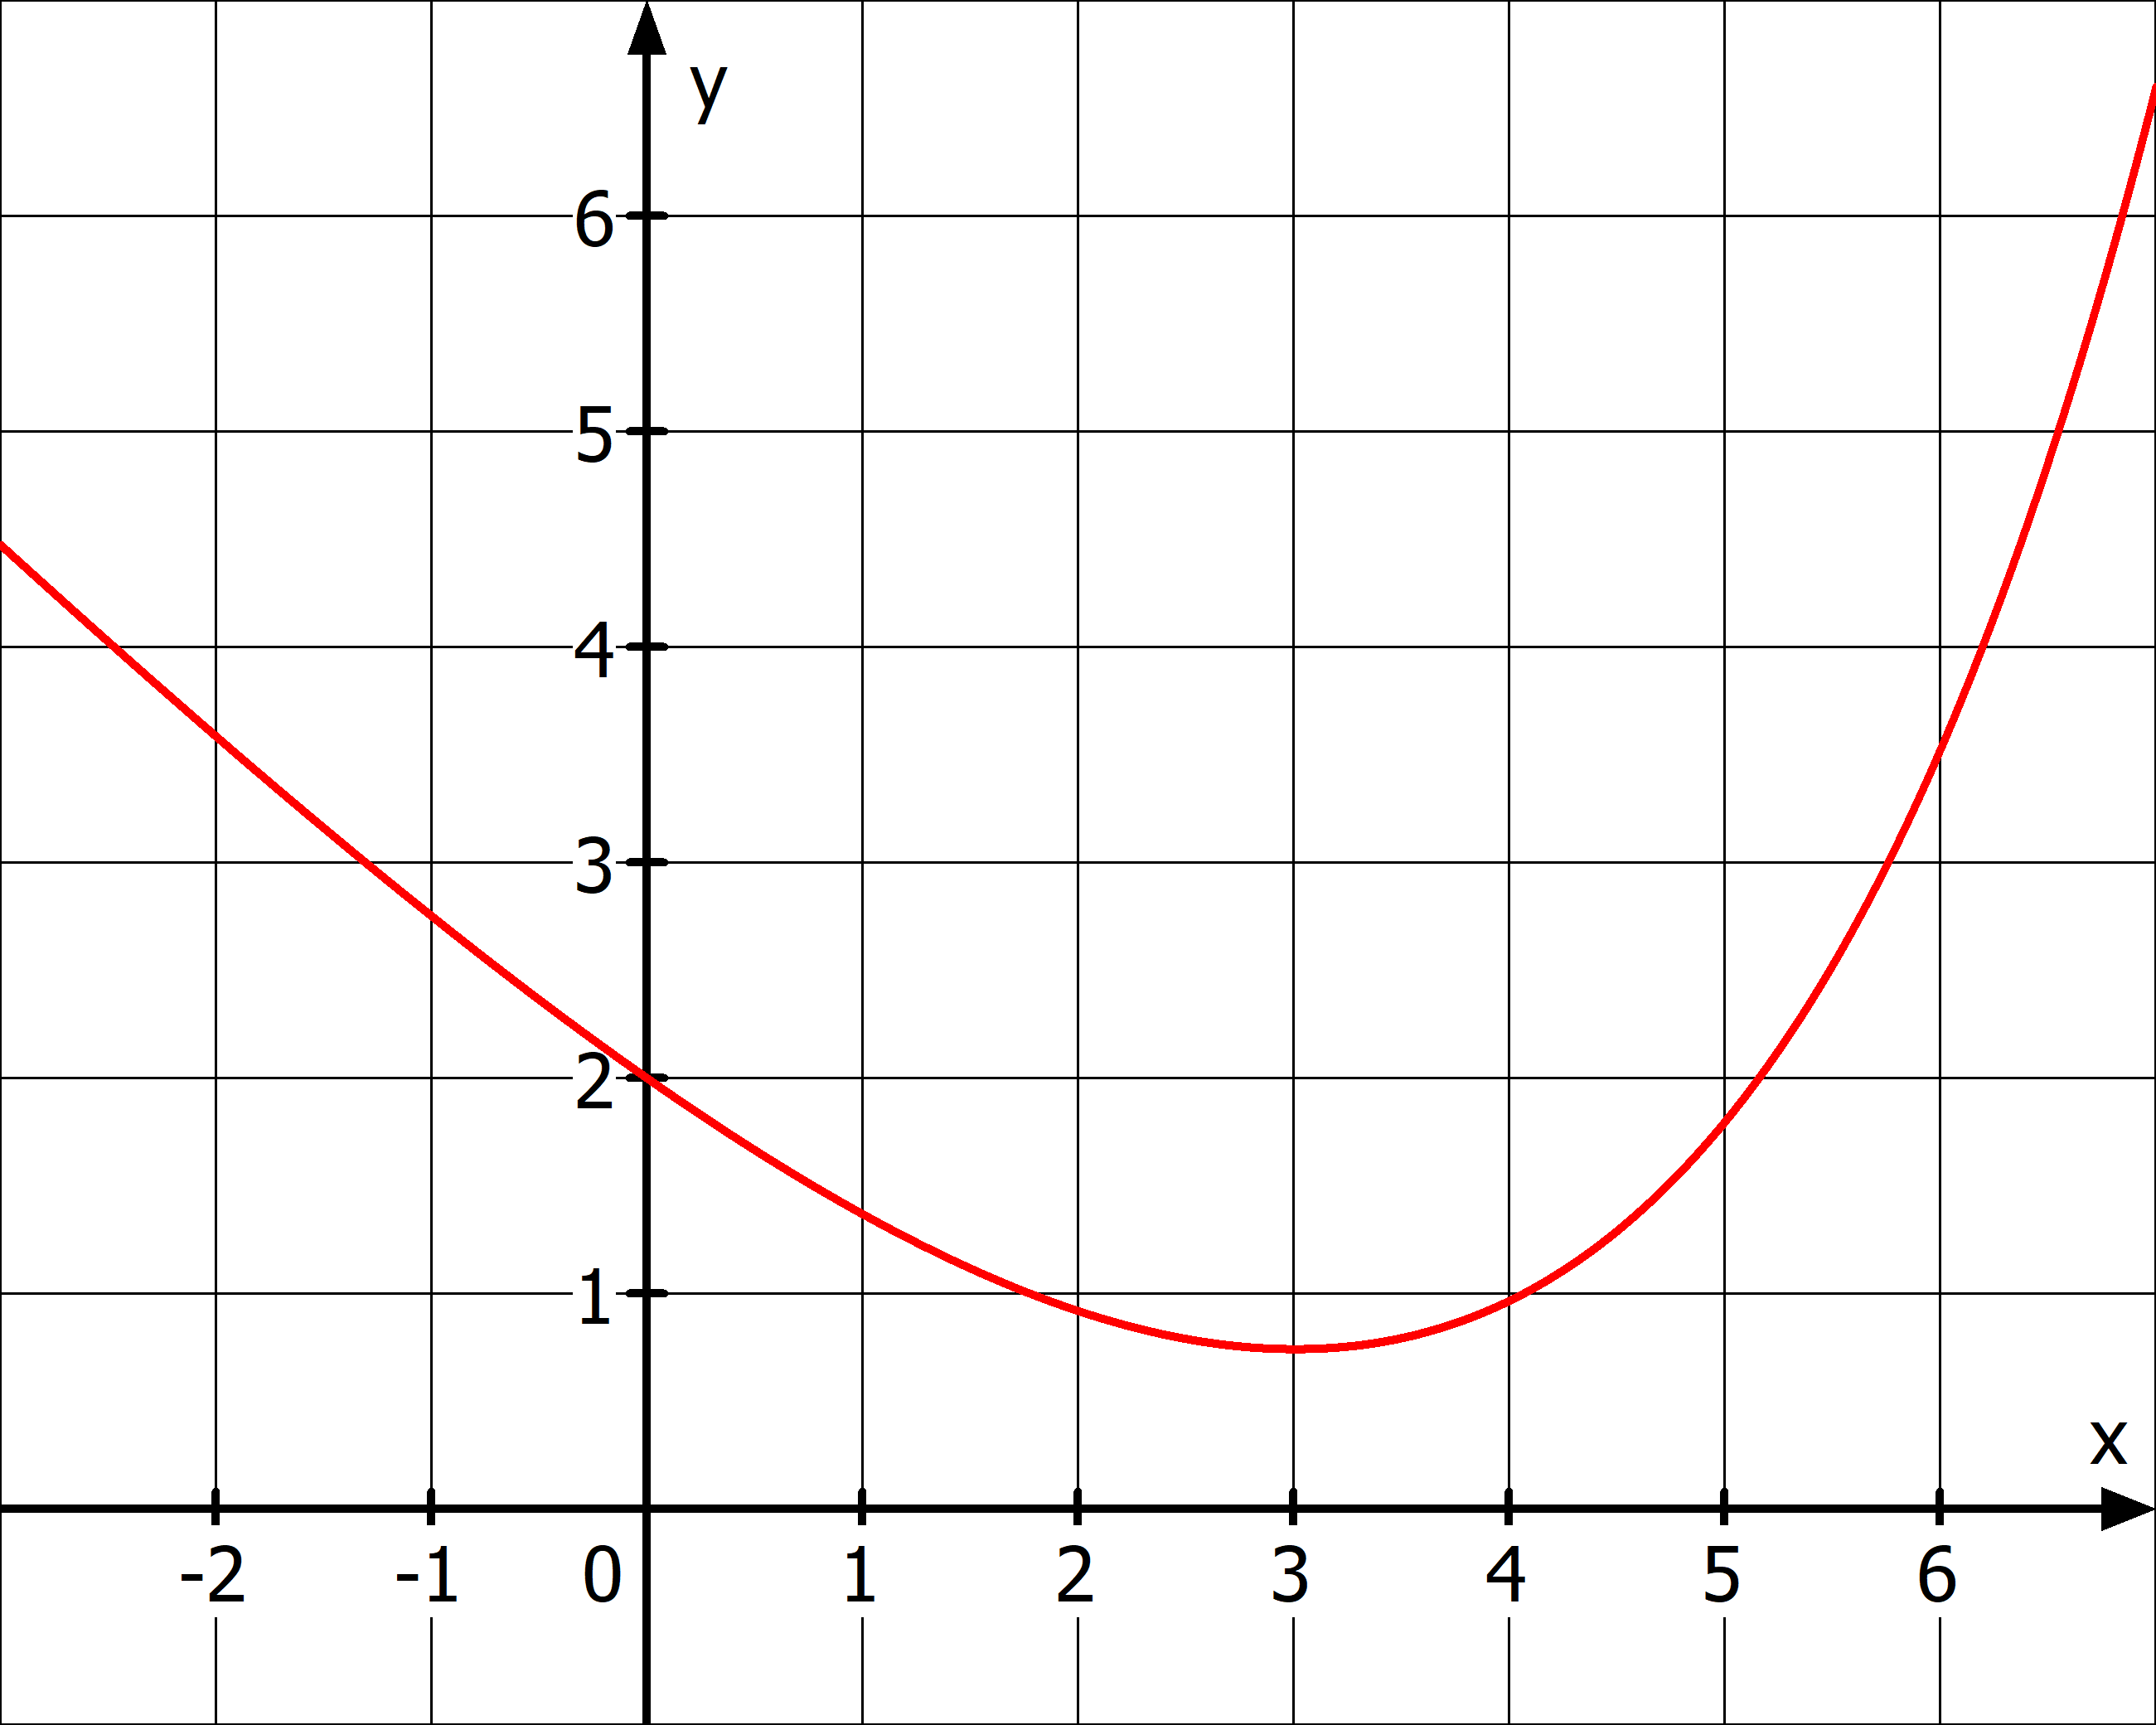
\includegraphics[width=\textwidth]{\eFkt/pics/VA_8.png}
        \end{minipage}}%

        \medskip

        \item Verschiebt man das Schaubild nur in \(y\)-Richtung, so genügt es das Schaubild um 2 Einheiten nach unten zu schieben:

        \(f_v(x)=0,75e^{0,4x}-x-0,75\)
    \end{enumerate}
\end{Answer}
\begin{Answer}[ref=eFktVA_9]

    Aus \(k(0)=3+0-6=-3<0\) und \(k(0,25)=3e+1-6=3e-5\approx8,1-5=3,1>0\) folgt auf Grund des Vorzeichenwechsels, dass die Funktion in diesem Intervall mindestens eine Nullstelle haben muss. (Es wurde die Näherung \(e\approx 2,7\) verwendet.)
\end{Answer}
\begin{Answer}[ref=eFktVA_10]
\begin{enumerate}[label=\alph*)]
    \item Zu Beginn des Experiments liegt der pH-Wert bei \(p(0)=13,5-6,5=7\) und nähert sich dann der Asymptoten bei \(y=13,5\) an. Das Messgerät muss also den Bereich zwischen 7 und 13,5 abdecken.
    \item Die Lösung ergibt sich aus folgender Gleichung
    \begin{align*}
        p(V)&=10\\
        13,5-6,5e^{-0,2V}&=10\ \vert\ -13,5\\
        -6,5e^{-0,2V}&=-3,5\ \vert\ :(-6,5)\\
        e^{-0,2V}&=\frac{7}{13}\ \vert\ \ln\\
        -0,2V&=\ln\left(\frac{7}{13}\right)\ \vert\ \cdot(-5)\\
        V&=-5\ln\left(\frac{7}{13}\right)\\
        V&\approx 3,10
    \end{align*}
    Es müssen also 3,10 mL Kalilauge hinzugefügt werden, um den Umschlagpunkt zu erreichen.
\end{enumerate}
\end{Answer}
\begin{Answer}[ref=eFktVA_11]
\begin{align*}
    e^{-2x}-4e^{-x}&=0\\
    e^{-x}\left(e^{-x}-4\right)&=0\ \vert\text{ SvN }e^{-x}=0\Lightning\text{ oder}\\
    e^{-x}-4&=0\ \vert\ +4\\
    e^{-x}&=4\ \vert\ \ln\\
    -x&=\ln(4)\ \vert\ \cdot(-1)\\
    x&=-\ln(4)
\end{align*}
\end{Answer}
\begin{Answer}[ref=eFktVA_12]
\begin{align*}
    2e^x-4&=e^x\ \vert\ -e^x+4\\
    e^x&=4\ \vert\ \ln\\
    x&=\ln(4)
\end{align*}
\end{Answer}
\begin{Answer}[ref=eFktVA_13]

\begin{minipage}{\textwidth}
    \adjustbox{valign=t, padding=0ex 0ex 2ex 0ex}{\begin{minipage}{.5\textwidth-2ex}
            Die Gleichung der Asymptoten ist \(y=-4\). Zum Zeichnen des Schaubildes die Wertetabelle des Taschenrechners verwenden!

            Das Schaubild müsste um 6 Einheiten nach oben verschoben werden, damit das verschobene Schaubild die Asymptote \(y_v=2\) hat.
    \end{minipage}}%
    \adjustbox{valign=t, padding=2ex 0ex 0ex 0ex}{\begin{minipage}{.5\textwidth-2ex}\centering
            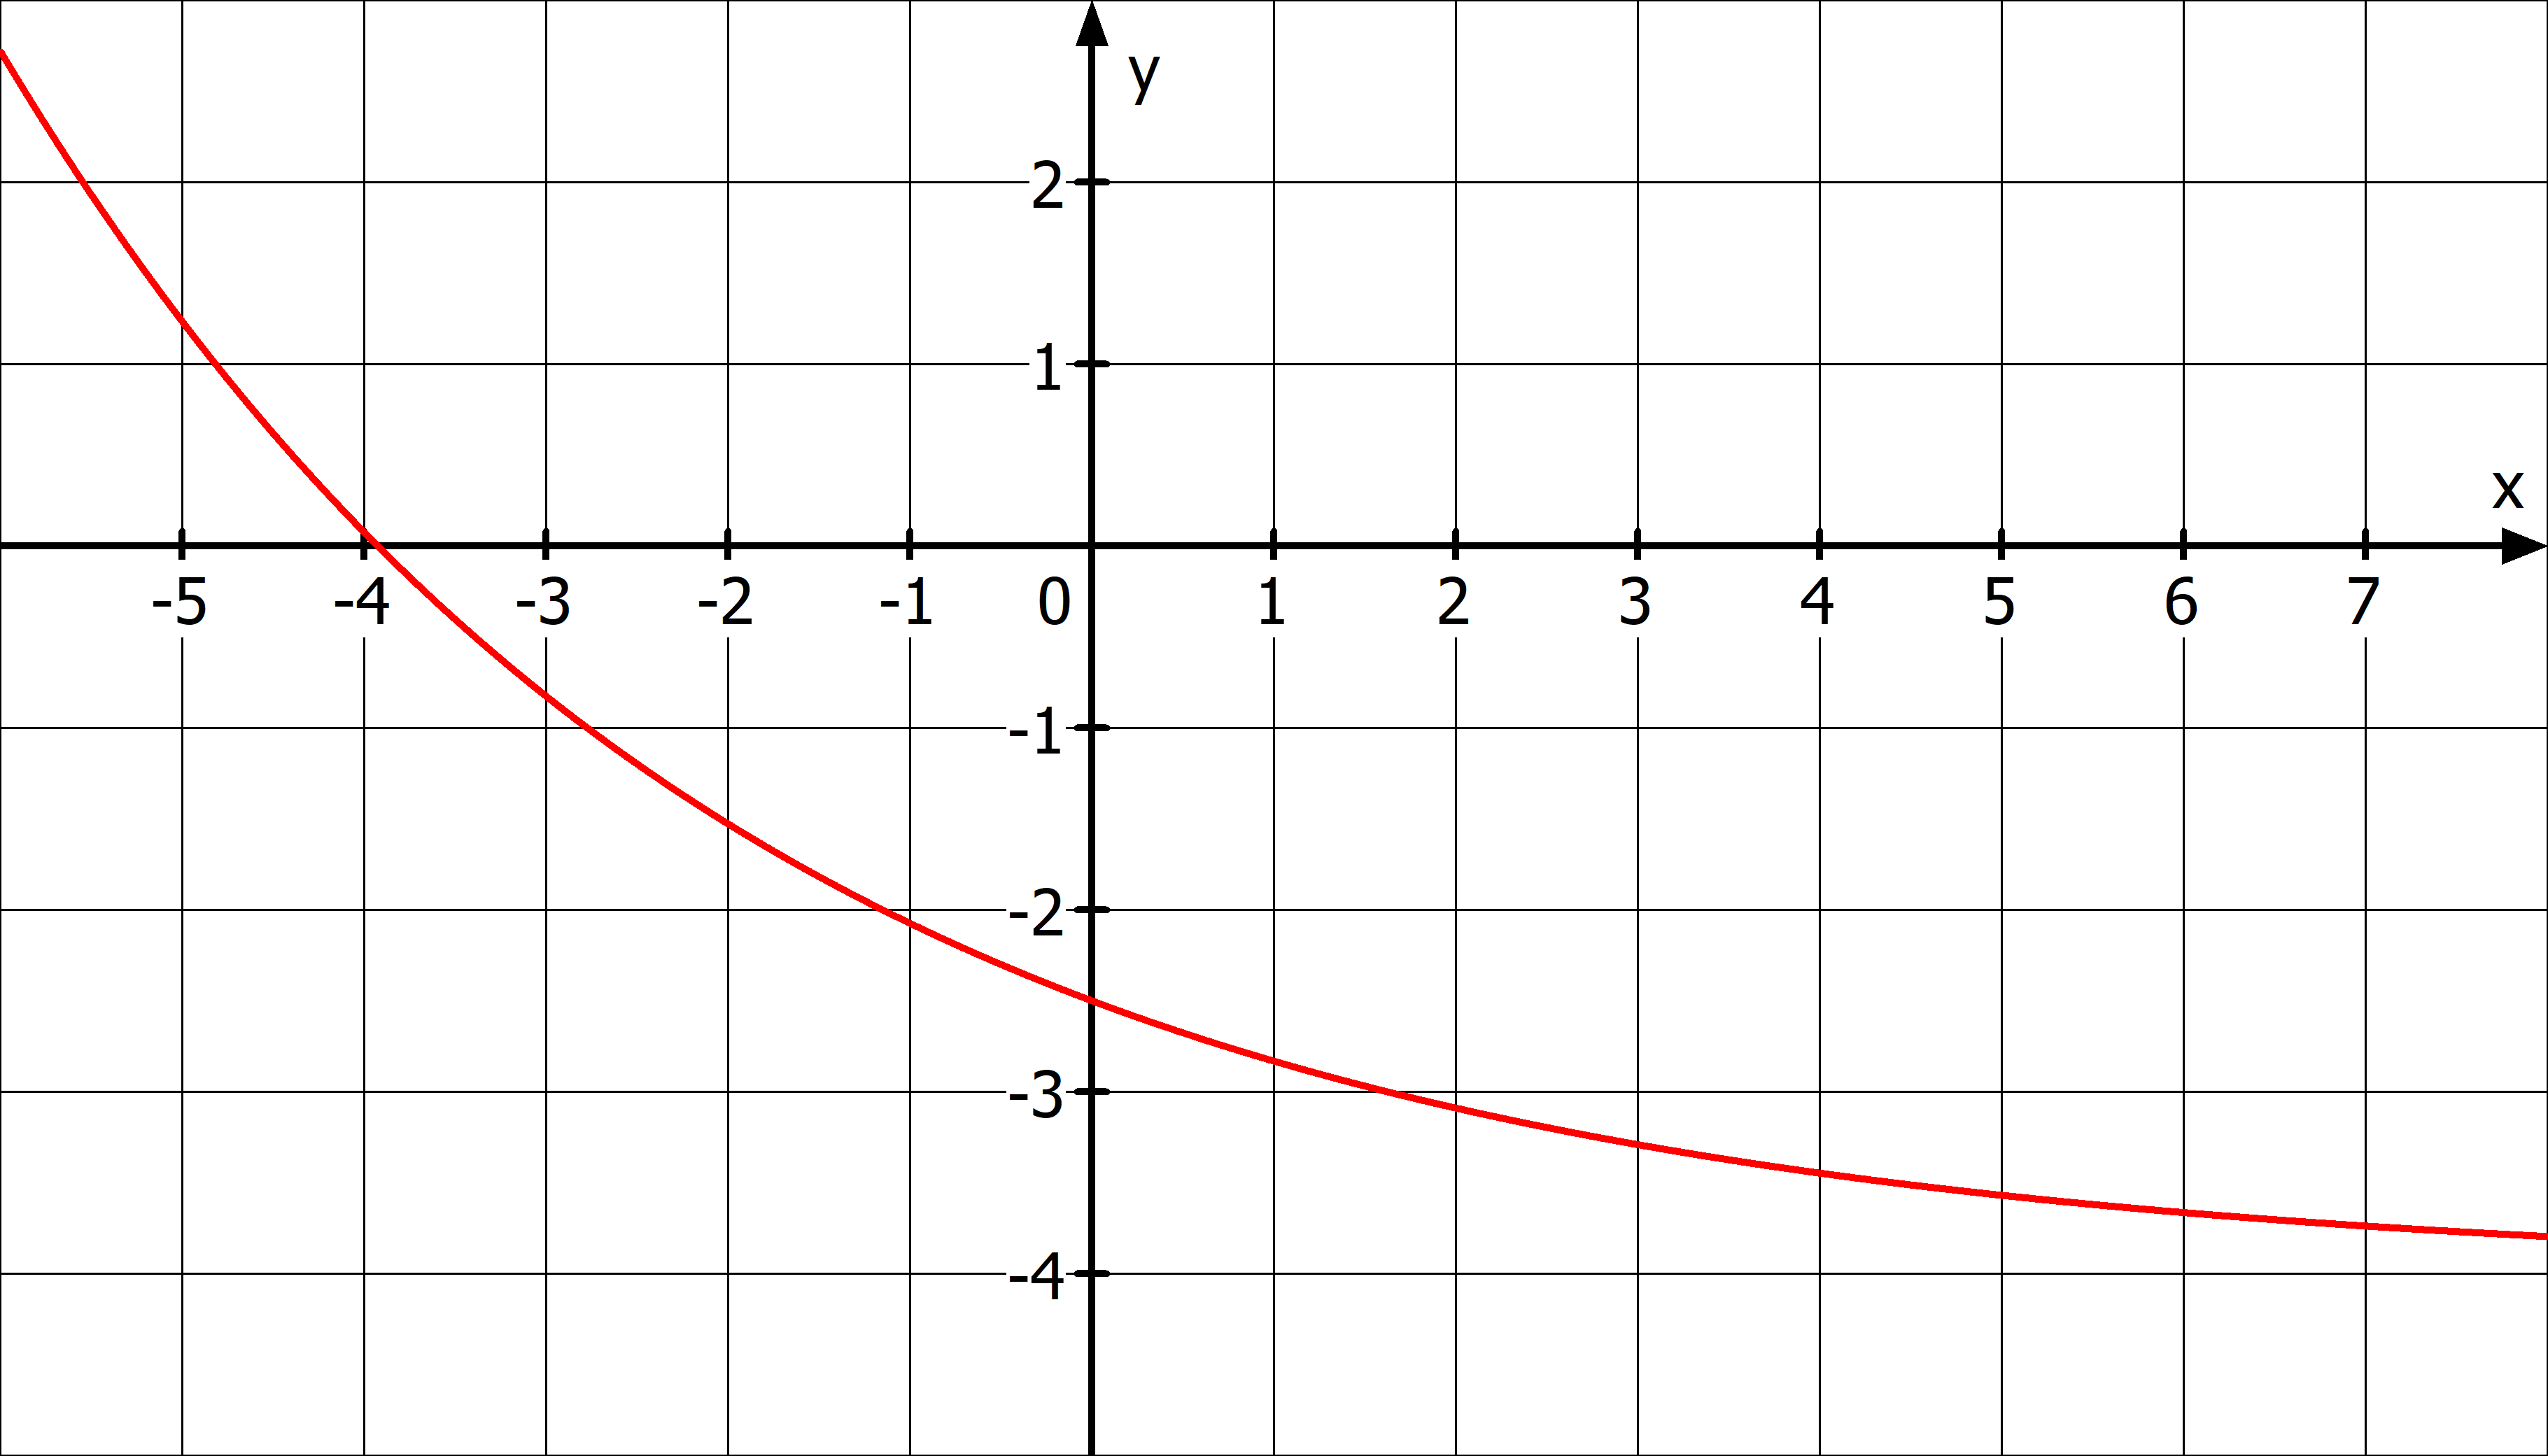
\includegraphics[width=\textwidth]{\eFkt/pics/VA_13.png}
    \end{minipage}}%
\end{minipage}
\end{Answer}
\begin{Answer}[ref=eFktVA_14]

Wir führen die Schritte rückwärts aus:

\(6e^{-2x}+4\xrightarrow{\text{3 Einheiten nach oben}}6e^{-2x}+7\xrightarrow{\text{mit Faktor 2 stauchen}}3e^{-2x}+3,5\)

Die gesuchte Funktion ist also \(g(x)=3e^{-2x}+3,5\)
\end{Answer}
\begin{Answer}[ref=eFktVA_15]

    \begin{minipage}{\textwidth}
        \adjustbox{valign=t, padding=0ex 0ex 2ex 0ex}{\begin{minipage}{.5\textwidth-2ex}
                \begin{enumerate}[label=\alph*)]
                    \item Die beiden Kaffee haben zum Zeitpunkt \(t=0\) die gleiche Temperatur. Mit \(a=97\) gilt \(T_1(0)=21+68=89=-8+97=T_2(0)\)
                    \setcounter{enumi}{2}
                    \item \(T_1\) beschreibt die Temperatur des Kaffees in der Wohnung, da dieser langsamer abkühlt und langfristig die Temperatur in der Wohnung von 21°C erreicht (Asymptote ist \(y_1=21\)). Dementsprechend beschreibt \(T_2\) die Temperatur des Kaffees im Außenbereich, da er schneller abkühlt und langfristig eine negative Temperatur von -8°C erreicht.
                \end{enumerate}
        \end{minipage}}%
        \adjustbox{valign=t, padding=2ex 0ex 0ex 0ex}{\begin{minipage}{.5\textwidth-2ex}\centering
                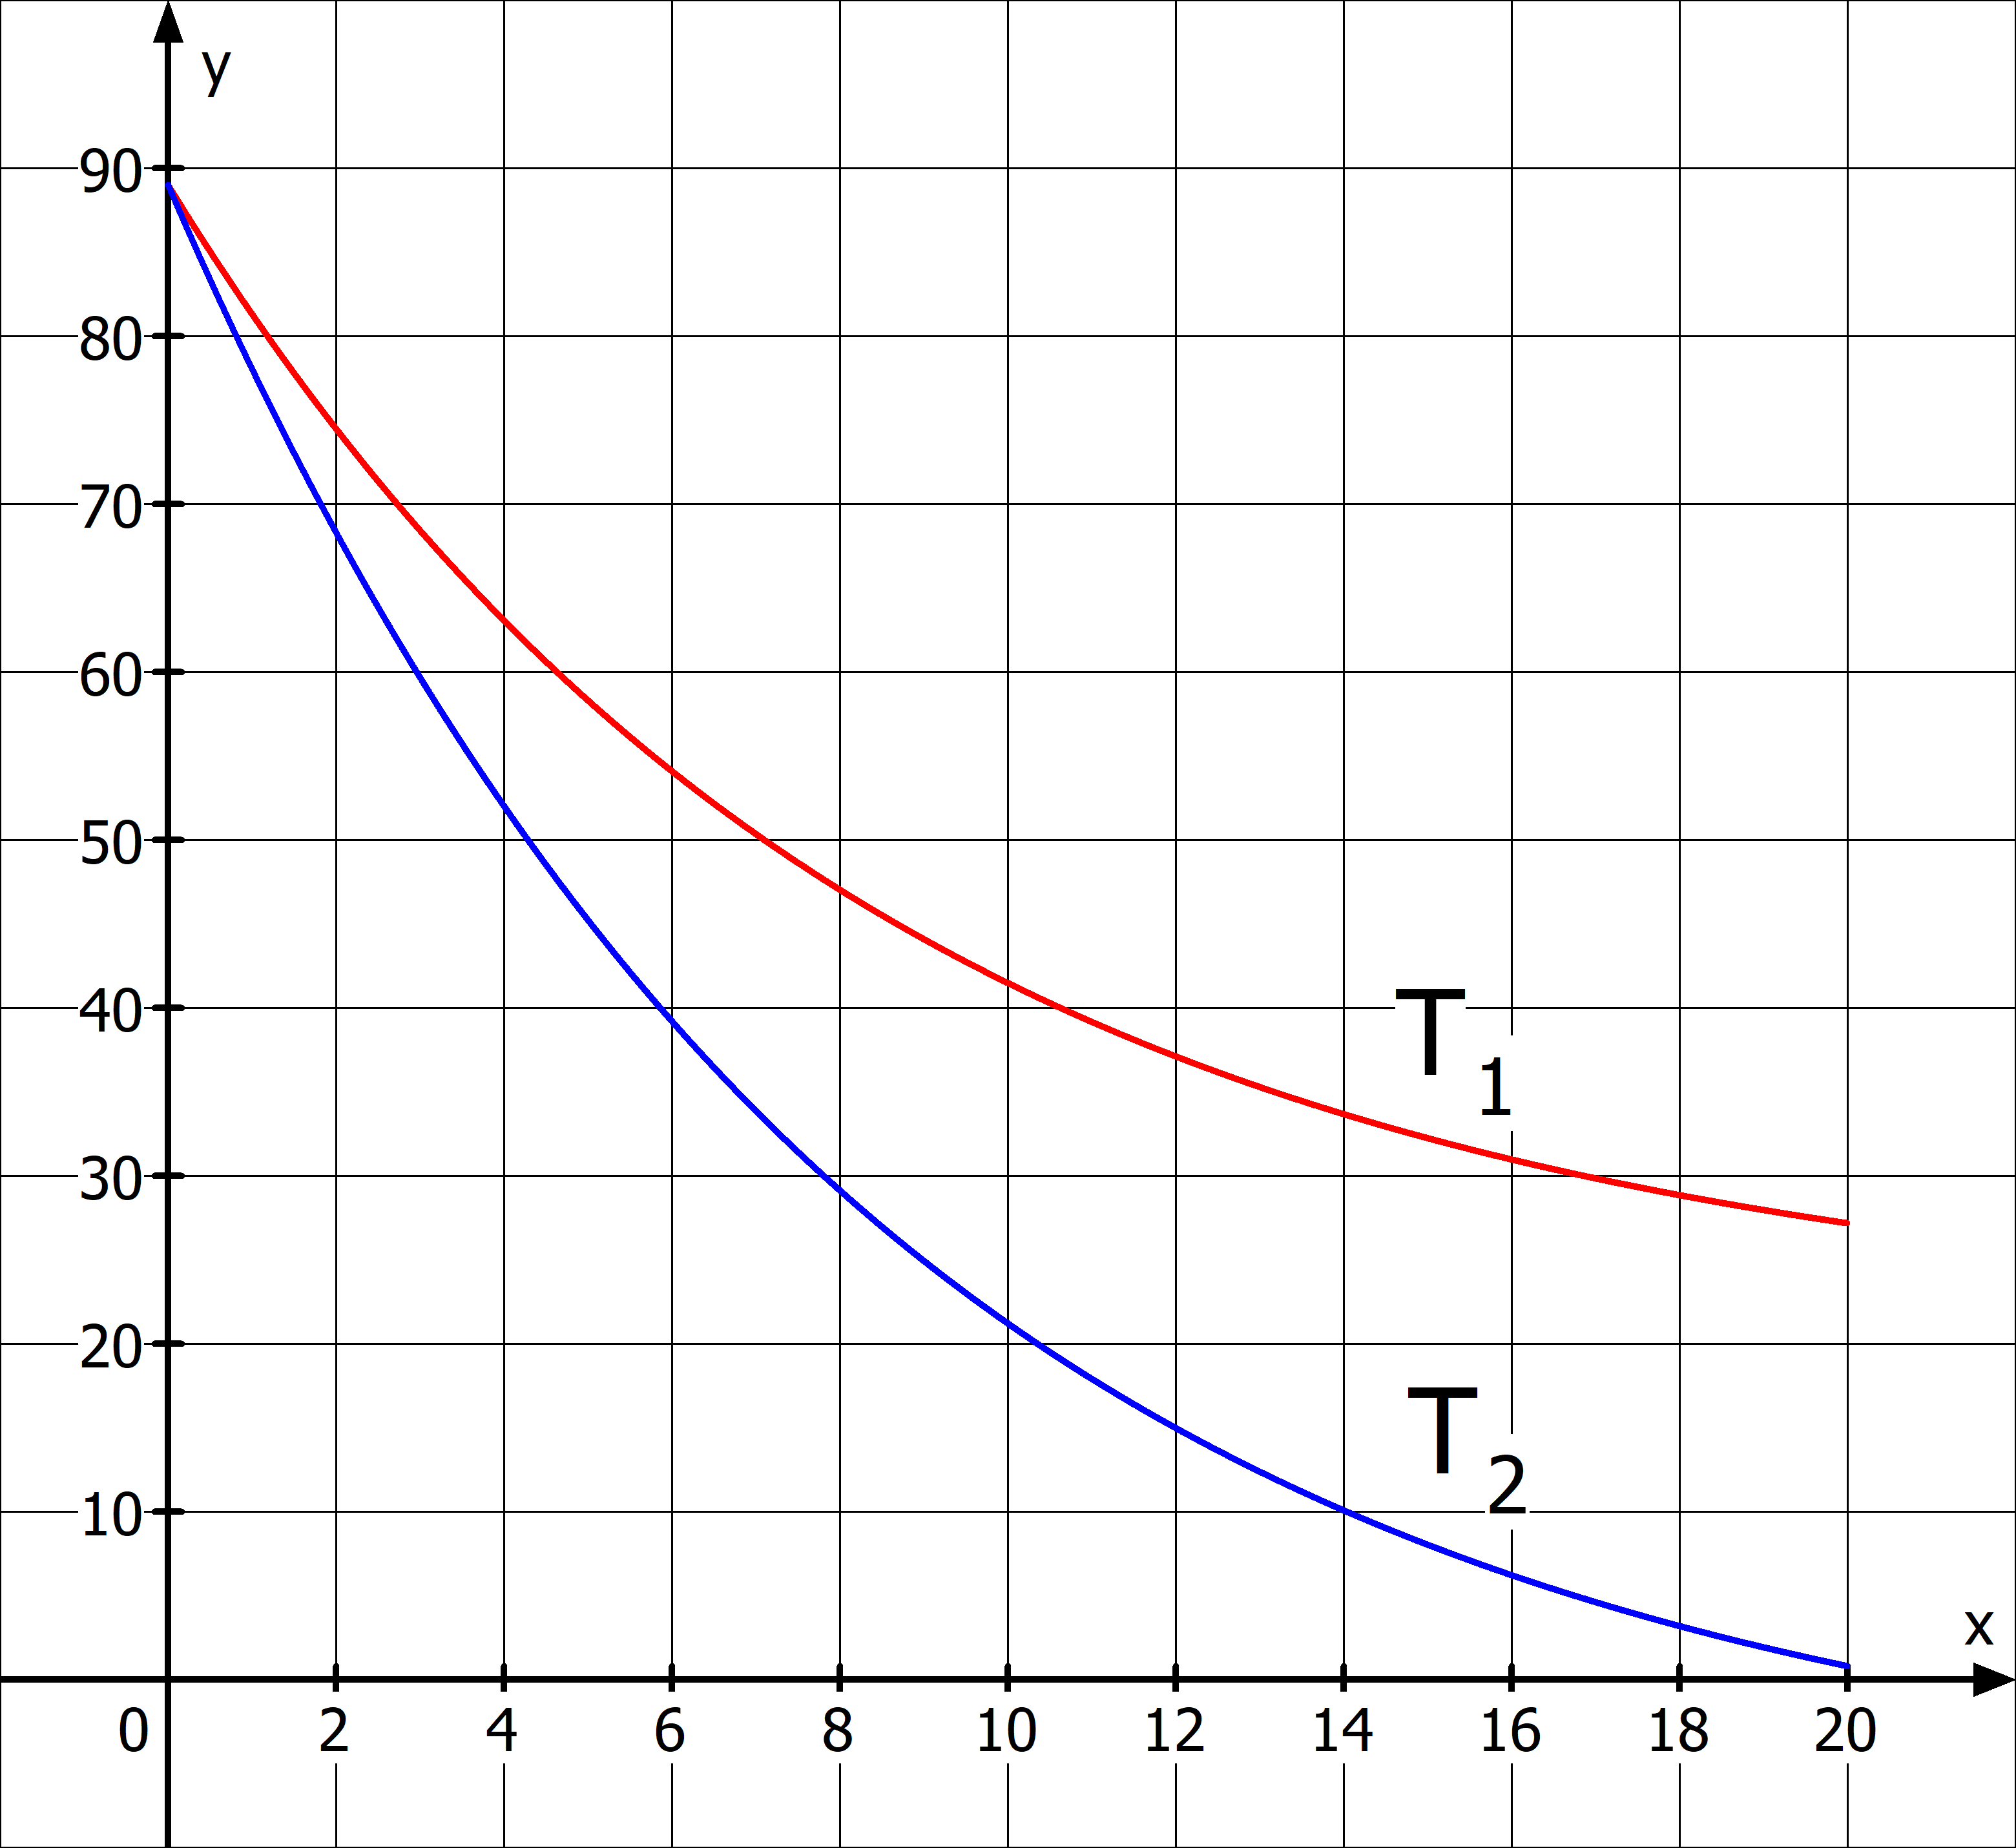
\includegraphics[width=\textwidth]{\eFkt/pics/VA_15.png}

                Wertetabelle des Taschenrechners verwenden!
        \end{minipage}}%
    \end{minipage}%

    \medskip

    \begin{enumerate}[label=\alph*)]
    \setcounter{enumi}{3}
    \item Man muss für beide Funktionen folgende Gleichungen lösen:

    \begin{minipage}{\linewidth}
        \adjustbox{valign=t}{\begin{minipage}{.5\textwidth}
                \begin{align*}
                    T_1(t)&=45\\
                    21+68e^{-0,12t}&=45\ \vert\ -21\\
                    68e^{-0,12t}&=24\ \vert\ :68\\
                    e^{-0,12t}&=\frac{6}{17}\ \big\vert\ \ln\\
                    -0,12t&=\ln\left(\frac{6}{17}\right)\ \big\vert\ :(-0,12)\\
                    t&\approx 8,68
                \end{align*}
        \end{minipage}}%
        \adjustbox{valign=t}{\begin{minipage}{.5\textwidth}
                \begin{align*}
                    T_2(t)&=45\\
                    -8+97e^{-0,12t}&=45\ \vert\ +8\\
                    97e^{-0,12t}&=53\ \vert\ :97\\
                    e^{-0,12t}&=\frac{53}{97}\ \big\vert\ \ln\\
                    -0,12t&=\ln\left(\frac{53}{97}\right)\ \big\vert\ :(-0,12)\\
                    t&\approx 5,04
                \end{align*}
        \end{minipage}}%
    \end{minipage}
    Eine Person kann ihren Kaffee also knapp 4 Minuten früher genießen (\(8,68-5,04=3,64\)).
\end{enumerate}
\end{Answer}